\documentclass[11pt]{standalone}
\usepackage{amssymb}
\usepackage{amsmath}
\usepackage[no-math]{fontspec}
\usepackage{unicode-math}
\usepackage{libertinus}
\usepackage{pgf,xcolor}
\usepackage{tikz}
\usetikzlibrary{arrows.meta, backgrounds}
\usepackage{pgfplots}
\pgfplotsset{compat=newest}

\definecolor{my_darkgray}{HTML}{484949}
\definecolor{my_lightgray}{HTML}{F3F4F4}
\definecolor{my_darkblue}{HTML}{005A94}
\definecolor{my_lightblue}{HTML}{CCDEE9}
\definecolor{my_yellow}{HTML}{FFEC7F}
\definecolor{my_red}{HTML}{E60000}
\definecolor{my_orange}{HTML}{E87846}

\begin{document}
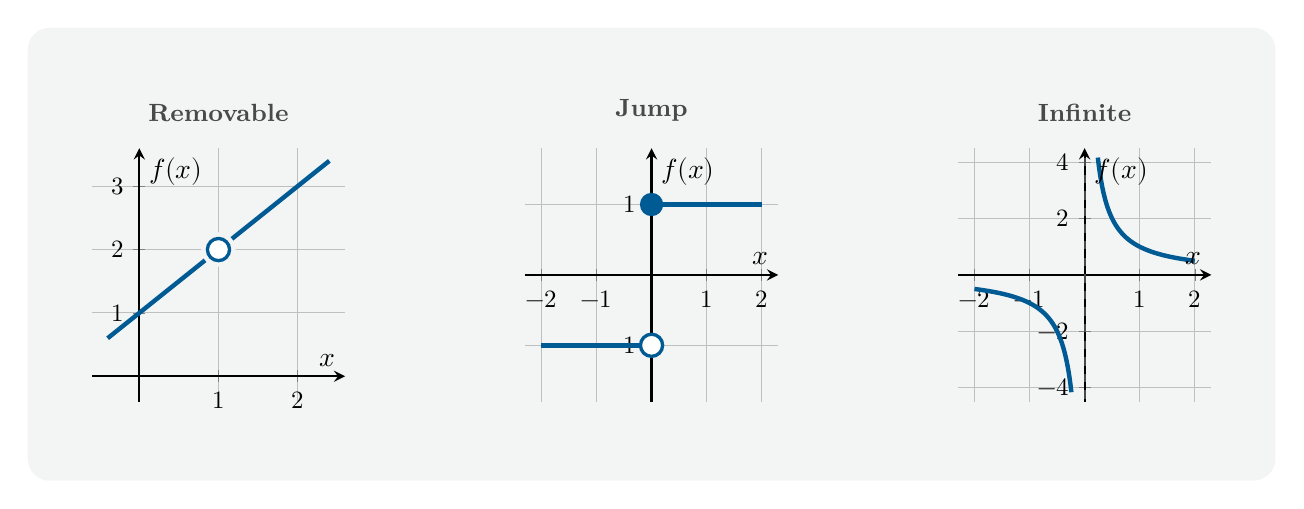
\begin{tikzpicture}[
    show background rectangle,
    background rectangle/.style={fill=my_lightgray, rounded corners=8pt},
    inner frame sep=0.8cm
]

%% ------------------------------------------------------------------
%% Sub-plot 1: Removable discontinuity
%%   f(x) = x + 1,  undefined at x = 1  (open circle at (1, 2))
%% ------------------------------------------------------------------
\begin{axis}[
    name=ax1,
    at={(0cm, 0cm)}, anchor=south west,
    width=4.8cm, height=4.8cm,
    axis lines=center,
    xlabel={$x$},
    ylabel={$f(x)$},
    grid=both,
    axis line style={thick},
    xmin=-0.6, xmax=2.6,
    ymin=-0.4, ymax=3.6,
    xtick={-0, 1, 2},
    ytick={1, 2, 3},
    tick label style={font=\small},
    title={\small Removable},
    title style={font=\small\bfseries, text=my_darkgray},
    clip=false,
]

%% Line  y = x + 1,  split at the hole so the gap is visible
\addplot[draw=my_darkblue, ultra thick, domain=-0.4:0.93]{ x + 1 };
\addplot[draw=my_darkblue, ultra thick, domain=1.07:2.4]{ x + 1 };

%% Erase the point on the line at (1, 2) with a white-filled circle
\addplot[only marks, mark=*, mark size=6pt,
    mark options={draw=my_lightgray, fill=my_lightgray}]
    coordinates {(1, 2)};

%% Open circle at (1, 2) indicating the missing point
\addplot[only marks, mark=*, mark size=4pt,
    mark options={draw=my_darkblue, fill=white, line width=1.2pt}]
    coordinates {(1, 2)};

\end{axis}

%% ------------------------------------------------------------------
%% Sub-plot 2: Jump discontinuity
%%   f(x) = -1 for x < 0  (open circle at (0,-1))
%%   f(x) =  1 for x >= 0 (filled circle at (0, 1))
%% ------------------------------------------------------------------
\begin{axis}[
    name=ax2,
    at={(5.5cm, 0cm)}, anchor=south west,
    width=4.8cm, height=4.8cm,
    axis lines=center,
    xlabel={$x$},
    ylabel={$f(x)$},
    grid=both,
    axis line style={thick},
    xmin=-2.3, xmax=2.3,
    ymin=-1.8, ymax=1.8,
    xtick={-2, -1, 1, 2},
    ytick={-1, 1},
    tick label style={font=\small},
    title={\small Jump},
    title style={font=\small\bfseries, text=my_darkgray},
    clip=false,
]

%% Lower branch:  f(x) = -1 for x < 0
\addplot[draw=my_darkblue, ultra thick, domain=-2:0]{ -1 };

%% Upper branch:  f(x) = 1 for x >= 0
\addplot[draw=my_darkblue, ultra thick, domain=0:2]{ 1 };

%% Open circle at (0, -1): left-side limit, not the function value
\addplot[only marks, mark=*, mark size=4pt,
    mark options={draw=my_darkblue, fill=white, line width=1.2pt}]
    coordinates {(0, -1)};

%% Filled circle at (0, 1): the actual function value f(0) = 1
\addplot[only marks, mark=*, mark size=4pt,
    mark options={draw=my_darkblue, fill=my_darkblue}]
    coordinates {(0, 1)};

\end{axis}

%% ------------------------------------------------------------------
%% Sub-plot 3: Infinite discontinuity
%%   f(x) = 1/x,  vertical asymptote at x = 0
%% ------------------------------------------------------------------
\begin{axis}[
    name=ax3,
    at={(11.0cm, 0cm)}, anchor=south west,
    width=4.8cm, height=4.8cm,
    axis lines=center,
    xlabel={$x$},
    ylabel={$f(x)$},
    grid=both,
    axis line style={thick},
    xmin=-2.3, xmax=2.3,
    ymin=-4.5, ymax=4.5,
    xtick={-2, -1, 1, 2},
    ytick={-4, -2, 2, 4},
    tick label style={font=\small},
    title={\small Infinite},
    title style={font=\small\bfseries, text=my_darkgray},
    restrict y to domain=-4.4:4.4,
    clip=true,
]

%% Left branch of  f(x) = 1/x,  x < 0
%% (split before the singularity; restrict y is a safety net)
\addplot[draw=my_darkblue, samples=150, ultra thick, domain=-2:-0.24]
    { 1/x };

%% Right branch of  f(x) = 1/x,  x > 0
\addplot[draw=my_darkblue, samples=150, ultra thick, domain=0.24:2]
    { 1/x };

%% Vertical asymptote at x = 0
\draw[dashed, thick, draw=my_darkgray]
    (axis cs:0, -4.4) -- (axis cs:0, 4.4);

\end{axis}

\end{tikzpicture}
\end{document}
